
\section{Design Approach}

Function oriented design approach is comprised of many smaller sub-systems known as functions. These functions are capable of performing significant task in the system. The system is considered as top view of all functions.
Function oriented design inherits some properties of structured design where divide and conquer methodology is used.\\

This design mechanism divides the whole system into smaller functions, which provides means of abstraction by concealing the information and their operation. These functional modules can share information among themselves by means of information passing and using information available globally.\\

This design mechanism divides the whole system into smaller functions, which provides means of abstraction by concealing the information and their operation.. These functional modules can share information among themselves by means of information passing and using information available globally.\\

Function oriented design follows a top-down approach. This technique is mainly used for computation sensitive application. In this approach the state information is often represented in a centralized shared memory. It views system as Black Box that performs high level function and later decompose it detailed function so to be mapped to modules.
Design approach for student performance investigation is function-oriented. Basic emphasis is on replacing existing semi-automated system with an automated system. Following a function oriented design approach this system is divided into many smaller sub-systems like advisory, admin, graph creations, etc. These modules can share information with each other. 


\iffalse
 basic requirement of this app is that the user must be a system which contains an opertaion system such as windows, linux etc and have matlab installed in it. The minimum version of matlab is 2015 matlab version.


\noindent As shown in the Figure \ref{fig:1}, .\\Brief introduction showing the features available in the application.

\begin{figure}[ht]
\centering
\includegraphics[scale=0.5]{images/s1.png}
\caption{Screen 1}
\label{fig:1}
\end{figure}

\noindent This are the options the navigation drawer the app will contain. These will contain the screens the user can navigate too that can be seen in Figure \ref{fig:2}. \\

\begin{figure}[ht]
	\centering
	\includegraphics[scale=0.49]{images/s2.png}
	\caption{Screen 2}
	\label{fig:2}
\end{figure}

\noindent  Statistics will be able to change according to the dates selected. Default values will be the current week. User Will be able to see diagrams according to Quantity and
days, Quantity and categories and others.as seen in the Figure \ref{fig:3}.\\

\begin{figure}[ht]
\centering
\includegraphics[scale=0.5]{images/s3.png}
\caption{Screen 3}
\label{fig:3}
\end{figure}

\noindent Reminder view will contain details from the reminder created and the user can edit
the reminder values. in Figure \ref{fig:4}. \\

\begin{figure}[ht]
\centering
\includegraphics[scale=0.38]{images/s4.png}
\caption{Screen 4}
\label{fig:4}
\end{figure}

\noindent Reminder screen will show the current saved Reminder and if they are active or not.
To activate one it will have a switch next to the name so it can be activated in any
moment. The user will be able to erase and add from this view as seen in the Figure \ref{fig:5}. It's named as output.dxf. We can open that file in LibreCAD directly from the command-line.\\


\begin{figure}[ht]
\centering
\includegraphics[scale=0.5]{images/s6.png}
\caption{Screen 5}
\label{fig:5}
\end{figure}

\noindent Expenses View is the main screen that will be showed. The user will be able to add expenses and see a total amount in Today, Week and Month. as shown in Figure \ref{fig:6}. 

\begin{figure}[ht]
\centering
\includegraphics[scale=0.38]{images/s61.png}
\caption{Screen 6}
\label{fig:6}
\end{figure}

\noindent This activity will provide necessary help to the user. One can also mail the maker
(Gursimer Singh) for further queries as shown in Figure \ref{fig:7}. 

\begin{figure}[ht]
\centering
\includegraphics[scale=0.38]{images/s7.png}
\caption{Screen 7}
\label{fig:7}
\end{figure}
\noindent User will be able to add and delete categories from the Categories View \ref{fig:8}. 

\begin{figure}[ht]
\centering
\includegraphics[scale=0.38]{images/s8.png}
\caption{Screen 8}
\label{fig:8}
\end{figure}
\fi

\section{System Design}

	
	\subsection{Home}
	 User will see the home screen, which will be the introduction page of sports department.After that user will have access to the following parts : 
	\begin{itemize}
		\item \textbf{News Panel}:- This part is available in left side under student panel. Under this panel, user can view the latest news available in the sports deppartment published by the administrator.
		
		\item \textbf{Navigation bar}:- Navigation bar under student panel is different from the admin panel. Navigation bar in student panel has the following features : 
		\begin{itemize}
		\item Facilites : This part contains the faciliies available in the sports department such as foootball, hockey, cricket etc.
		\item Achievements : Under this portion, achievement of students under intramural, extramural and Ptu tournaments are acknowledge.
		\item Atheletic meet : Here, Recoords are maintained and best athletes are acknowledge.
		\item Commitee : Under this portion, commitee members of the sports department are mentioned.
\end{itemize}		   
				
		\item \textbf{Navigation bar(admin)}:- Navigation bar in the admin panel contains following options:
		\begin{itemize}
			\item Facilites : This part contains the faciliies available in the sports department such as foootball, hockey, cricket etc.
			
			\item \textbf{Commitee}:- It shows the list of commitee members currently available in the sports department.
			
		
		\item Atheletic meet : Here, Recoords are maintained and best athletes are acknowledge.
		\item Vision : Vision of the sports department is disscused under this portion. 
		\item Logout : To get looged out from the admin panel.
			
			\item{Achievement}:-It will have two options:
			\begin{itemize} 
			\item \textbf{Intramural}:-Achievement of students who participated or got medals in activities or events performed under college boundaries will be displayed here.
			\item \textbf{Extramural}:-Achievement of students who participated or got medals in activities or events performed outside of college boundaries will be displayed here.
			\item \textbf{PTU Stars}:- Achievement of students who participated in the sports events organized by the PTU.
			  \item \textbf{Intervarsity}:-Achievement of students who participated at university level.
			
			
			\end{itemize}
			
			
		\end{itemize}
	\end{itemize}
\newpage
\section{System Design}

\begin{figure}[ht]
	
	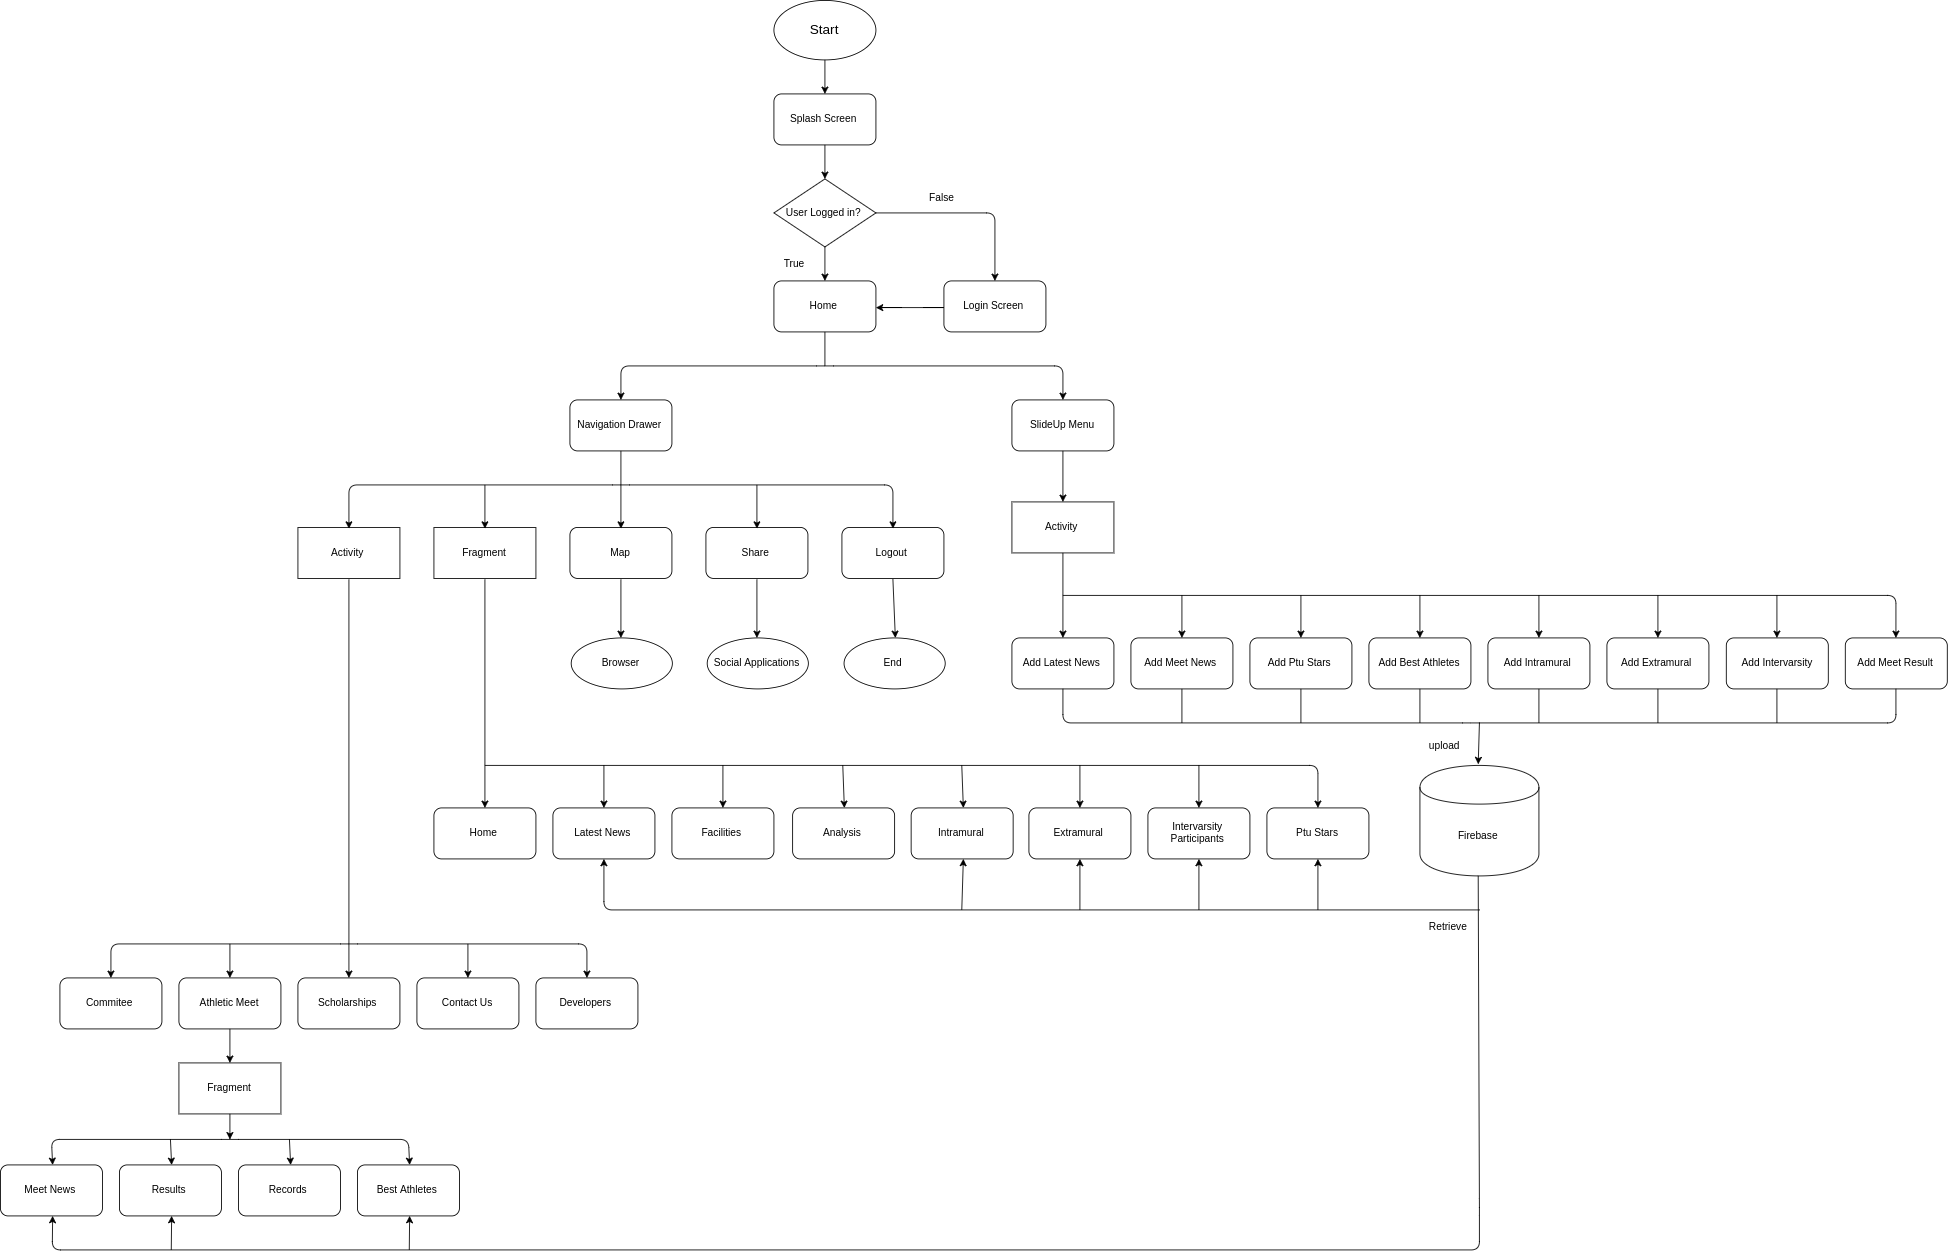
\includegraphics[scale=0.26]{images/Gndecadmingne.png}
	\caption{Flow Chart of gndec admin}
\end{figure}

\newpage
\begin{figure}[ht]
	
	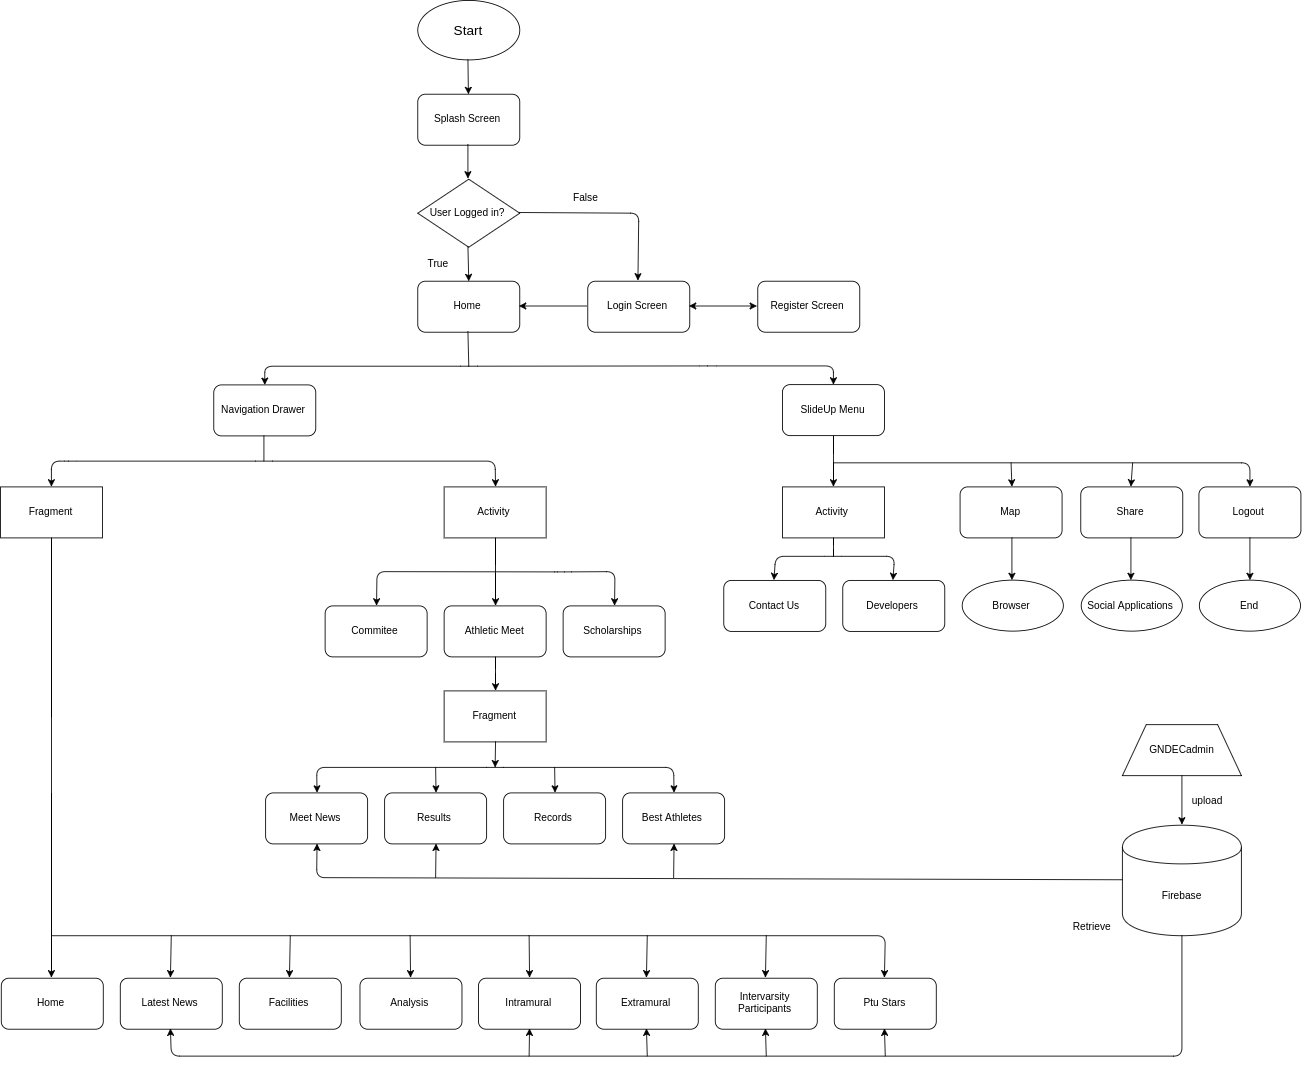
\includegraphics[scale=0.35]{images/Gndecstudent.png}
	\caption{Flow Chart of gndec student}
\end{figure}



\newpage
\section{Database Design}

	\subsection{ER Diagram}
	
	
	\begin{figure}[ht]
		\centering
		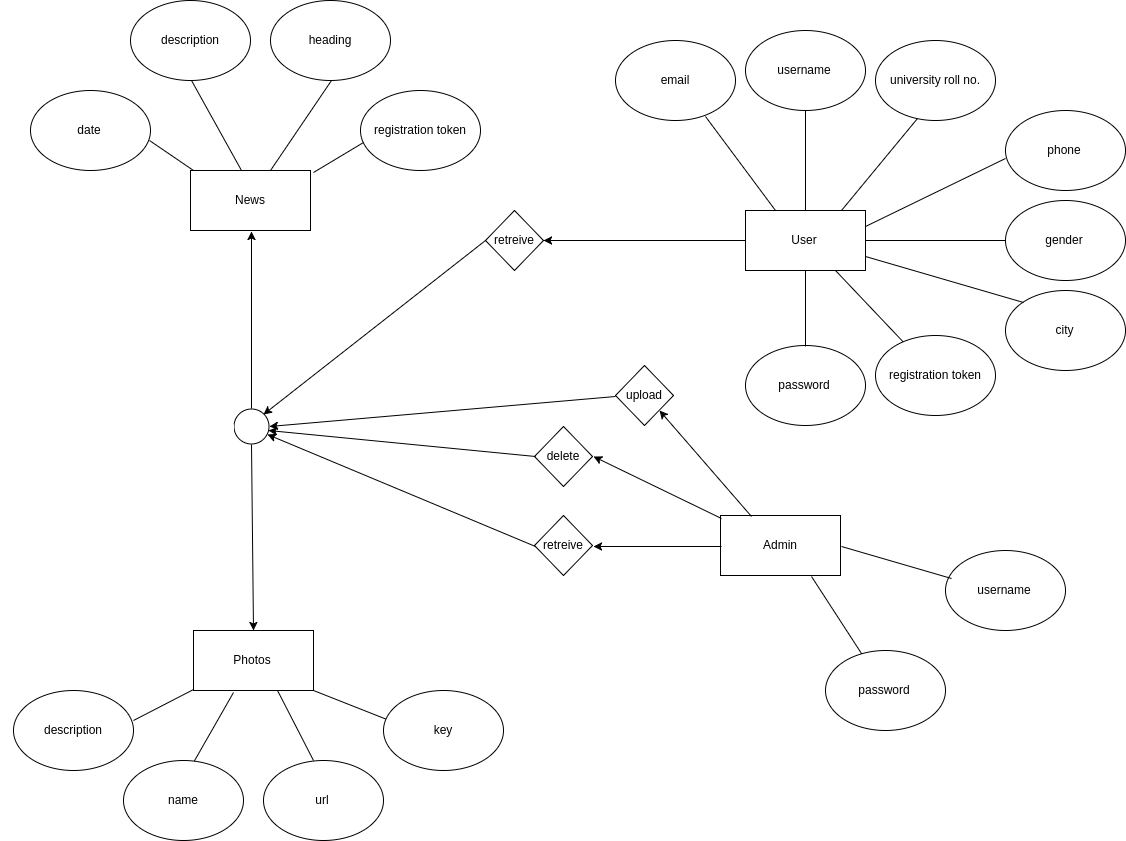
\includegraphics[scale=0.35]{images/ergndec.png}
		\caption{ER Diagram}
	\end{figure}
	
	\subsection{Database Connection Controls and Strings}
	The Firebase Realtime Database is a cloud-hosted database. Data is stored as JSON and synchronized in realtime to every connected client. When we build cross-platform apps with our iOS, Android, and JavaScript SDKs, all of our clients share one Realtime Database instance and automatically receive updates with the newest data. \\
	
	It is recommended using the Firebase Assistant to connect your app to Firebase. The Firebase Assistant can connect our existing project or create a new one for us and automatically install any necessary gradle dependencies.\\

	
